In this section, we describe the different provisioning methods implemented in ConPaaS.



\subsection{Naive provisioning}

The existing infrastructures offer provisioning mechanism that adjust the amount of resources depending on the load of the currently allocated resources. Within this group of provisioning mechanisms, we include the simple trigger-based systems that define threshold rules to increase and decrease the computational power of an application in order to guarantee several performance requirements. As an example, the Auto Scaling system offered by Amazon EC2~\cite{amazonEC2} scales out an application whenever its CPU usage in the last 10min exceeds a specific threshold (Amazon recommends values from 70\%).  This rules-based method is currently used in mature cloud platforms such as RightScale~\cite{right-scale} or OpenShift~\cite{openshift}. In ConPaaS, we also decided to offer a trigger-based provisioning mechanism, called "naive provisioning", that monitors CPU usage and response time thresholds. 

% , expressed in the form of a Service Level Agreement

Even though these type of mechanisms are simple and widely used in cloud platforms, they are naive and excessive reactive due to several factors: 

%regarding the decision making process

\begin{itemize}
\item  When hosting a web application, the system performance behavior fluctuates following an irregular pattern caused by the web traffic (workload). 

%Obviously, a reactive algorithm can be seen a good choice for resource provisioning, however. The system %performance of an application change in time if the type of workload changes.

\item Excessive reactive system can affect the system performance when handling flash crowds. A high frequency of scaling operations can provokes sharp and sudden fluctuations that affect the performance instead of improving it. So, it is particularly difficult to decide when to scale out or back. 

\item Services are handled as black boxes, the definition of threshold rules only covers system-level constraints such as response time and CPU usage. Therefore, when provisioning web applications, constraints such as request rate of static/non-static files may be also taken into consideration.

% when handling web traffic.

%These constraints are too generic, as other application-specific constraints are not considered. 

%\item VMs are heterogeneous in performance, and thereby their throughput vary depending of its hardware configuration (instance's types). 
\item The performance of virtual instances provided by current Clouds is largely heterogeneous, even when requesting the exact same type of instance each time \cite{ec2Performance}. 

% The provisioning mechanism omit the heterogeneity of the VMs associated to host an application. 

\end{itemize}

Based on these factors, we believe trigger-based provisioning mechanisms can be improved without drastically increasing its complexity. A solution seems to be the utilization of techniques that handle web application workload, while its implementation remains a simple exercise. In the following we present two algorithms that aims at solving these drawbacks by relying on more predictive and dynamic methods.

% to dynamically adjust the computational power to irregular workload pattern of web applications.


%previous knowledge about behavior of the application, avoid flash crowds too reactive
%and the definition of application-specific constraints 
%Tthe definition of threshold range based on how much workload a server can handle. what is the request %rate that a server can sustain without becoming overloaded?
%what is the value of the CPU utilization/load that indicates that a server is
%overloaded? These values are different from one application to another, and also
%from one server to another. 


%Second experiment: improved the basic provisioning with some application knowledge
%observed empirically (the maximum request rate we can send to a server, maybe also
%the maximum CPU utilization we can allow). The results show more stability in the
%provisioning.  


\subsection{History-aware provisioning}
Based on our previous knowledge from naive provisioning, we designed and implemented a more predictive and dynamic algorithm to handle temporal bursty workload. To achieve that, our algorithm relies on three simple techniques: weight-values for SLA constraints, flexible thresholds and  estimation of the workload trend. 

%In order to handle temporal bursty workload, we designed and implemented a predictive and reactive algorithm by relying on

\textbf{Weight-values:} once the system collected the monitoring data from application-specific constraints such as the CPU usage, response time and request rate for both non-static/static files. Traditional algorithms would scale out and back whenever CPU usage or response time values  exceed a beforehand defined threshold range. Nevertheless,  through the definition of weight values, our algorithm gives different priorities to each constraint when making decisions. 
Considering web applications, our method associate weight-values in an ascending order to the following constraints: request rate, cpu usage and response time. Accordingly the response time has a higher weight value than the request rate, since a high value in the response time rapidly indicate the existence of a performance degradation in a web application. High values in the request rate cannot always indicate that an application is becoming overloaded, due to the large diversity in the complexity of the requests.

\textbf{Flexible thresholds:} The history-aware algorithm establishes two types of threshold ranges: \emph{predictive} and \emph{reactive}. A \emph{predictive threshold} comprises a range of values that alert of possible workload alterations in advance. While a \emph{reactive threshold} comprises a range of values which are used to trigger scaling actions. As an example of CPU flexible threshold, we established a predictive range comprised between 30\% and 70\% , and a reactive comprised between 20\% and 80\%.  

\textbf{Workload's trend estimation:} Nowadays, there is a wide literature on mathematical models that try to predict future alterations in web application's workload. However, most models fail due to the irregular pattern of the web traffic, or its complexity to be utilized in real auto scaling systems. As a result, we decided to analyze the system performance behavior during an interval of time, thus avoiding flash crowds and slashdot effects. An exhaustive analysis of the monitoring data during a small interval of time (approx. during the last 20min) provides enough information to deduct the workload's trend, and thereby to classify the type of workload alteration as constant or temporal. Obviously, only constant variations may trigger scaling actions to avoid fluctuations in the system performance, as we will detail in Section~\ref{experiments}.

Using the history-aware algorithm we now collect application-specific metrics for our measurements, evaluate the evolution of the application workload avoiding an excessive reactive behavior, and handle threshold values that helps to predict possible SLA violations. Unfortunately, the heterogeneous nature of the VMs requires more dynamic provisioning algorithms. 

%In particular, the profiling techniques appears as a solution to tackle this problems of heterogeneity.


\section*{Profiling-based provisioning}

The heterogeneity of cloud platforms, and therefore, of their VMs affect to the accuracy of the provisioning decisions. VMs with better hardware configuration can sustain higher workload intensities. Based on that, each time ConPaaS requests a new VM from the Cloud, it must measure the individual performance profile of this particular VM instance before being able to decide what is the most efficient use of this resource. To do that, ConPaaS uses profiling techniques which represent a promisingly solution to this heterogeneity problem,  as we pointed out in ~\cite{jiangThesis}. 

\noindent There are two types of performance profiling: offline and online.

\begin{itemize}
\item \emph{Offline profiling} techniques gather information about VM instances to have an initial assessment of their throughput. This assessment will be used to predict SLA violations in advance. For instance, offline profiling can be used to define flexible threshold ranges for each VM (\emph{i.e.,} max. and min. request rate, etc...).

\item \emph{Online profiling} techniques enable to decide at runtime which set of VM instances is more suitable to handle the current workload intensity. Once the application started, online profiling can be also used to dynamically re-adjust the workload balance across VMs based on its own performance behavior. Specifically,  the profiling-based algorithm uses a mechanism to continuously adapt the online profile, in order to deal with possible changes in workload's type or in VMs performance. This online profile is used to dynamically adapt the load balancing weights and also our performance predictions. 

\end{itemize}

As illustrated on Figure~\ref{model}, we believe most existing problems in resource provisioning can be solved by combining the history-aware provisioning algorithm (referred as scaling on the Figure~\ref{model}) in conjunction with these two profiling techniques. The resulting provisioning system scales out/back an application utilizing all the benefits of heterogeneous cloud infrastructures in a predictive and dynamic manner.


%\fixme{unlike in some synthetic benchmarks, in Wikipedia there are large variations
%in the complexity of the articles; so the PHP processing time is more difficult 
% to predict}

\begin{figure}
\begin{center}
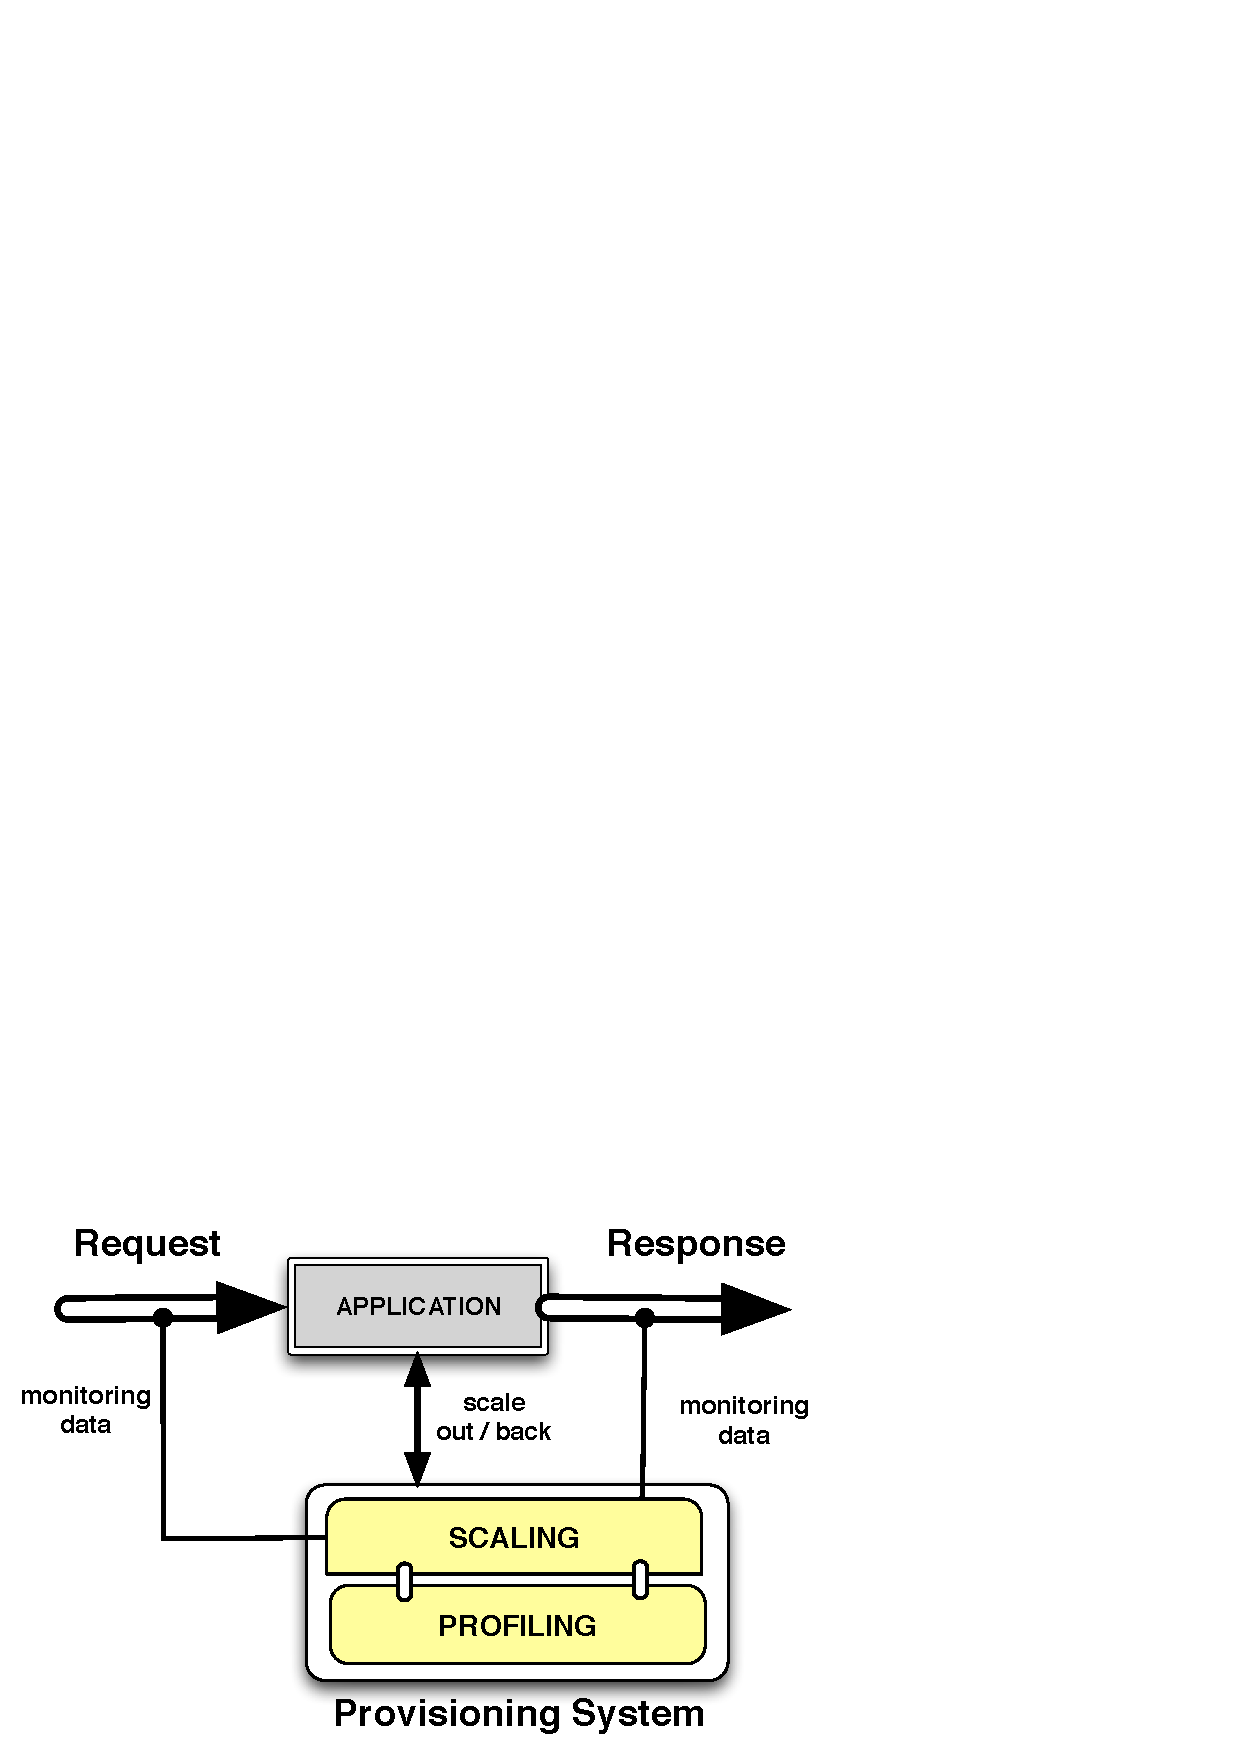
\includegraphics[width=0.4\textwidth, height=4cm]{./images/monitoringSchema.jpg}
\end{center}
\label{model}
\caption{Profiling Resource Provisioning}
\end{figure}
